\documentclass[serif]{beamer}
\usepackage{amsmath}
\usepackage{url}
\usepackage{bbm}
\usepackage{ucs}
\usepackage[utf8x]{inputenc}
\usepackage[ngerman]{babel}
\usepackage{color}
\usepackage{hyperref}
\usepackage{bookman}
\usepackage{nicefrac}
\usepackage{wasysym}

\usetheme{Boadilla}
\setbeamertemplate{footline}

\usecolortheme{lily}
\usefonttheme{serif}
\useinnertheme{circles}
\setbeamercovered{transparent}
\beamertemplatenavigationsymbolsempty

\definecolor{darkgreen}{rgb}{0,0.5,0}
\definecolor{purple}{HTML}{3333B2}

\hypersetup{
    bookmarks=true,
    unicode=true,
    pdftoolbar=true,
    pdfmenubar=true,
    pdffitwindow=false,
    pdfstartview={FitH},
    pdftitle={Stabilität invertierter Pendel},
    pdfauthor={Michael Hartmann},
    pdfsubject={Vortrag über Stabilität invertierter Pendel},
    pdfcreator={vim},
    pdfproducer={pdflatex},
    pdfkeywords={Mathieu} {Stabilität} {invertierte Pendel},
    pdfnewwindow=true,
    colorlinks=true,
    linkcolor=black,
    citecolor=green,
    filecolor=magenta,
    urlcolor=darkgreen
}



\title{Stabilität invertierter Pendel}
\institute{Kaffeeseminar}
\author{Michael Hartmann}
\date{4. November 2016}


\titlegraphic{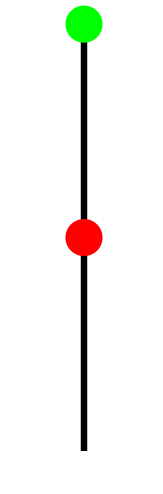
\includegraphics[scale=0.3]{images/title.png}}


\begin{document}

\begin{frame}
    \titlepage
\end{frame}


\frame{
    \frametitle{Überblick}
    \tableofcontents
}


\section{Einleitung}

\frame {
    \frametitle{Invertierte Pendel}

    \begin{center}
    \only<1> { 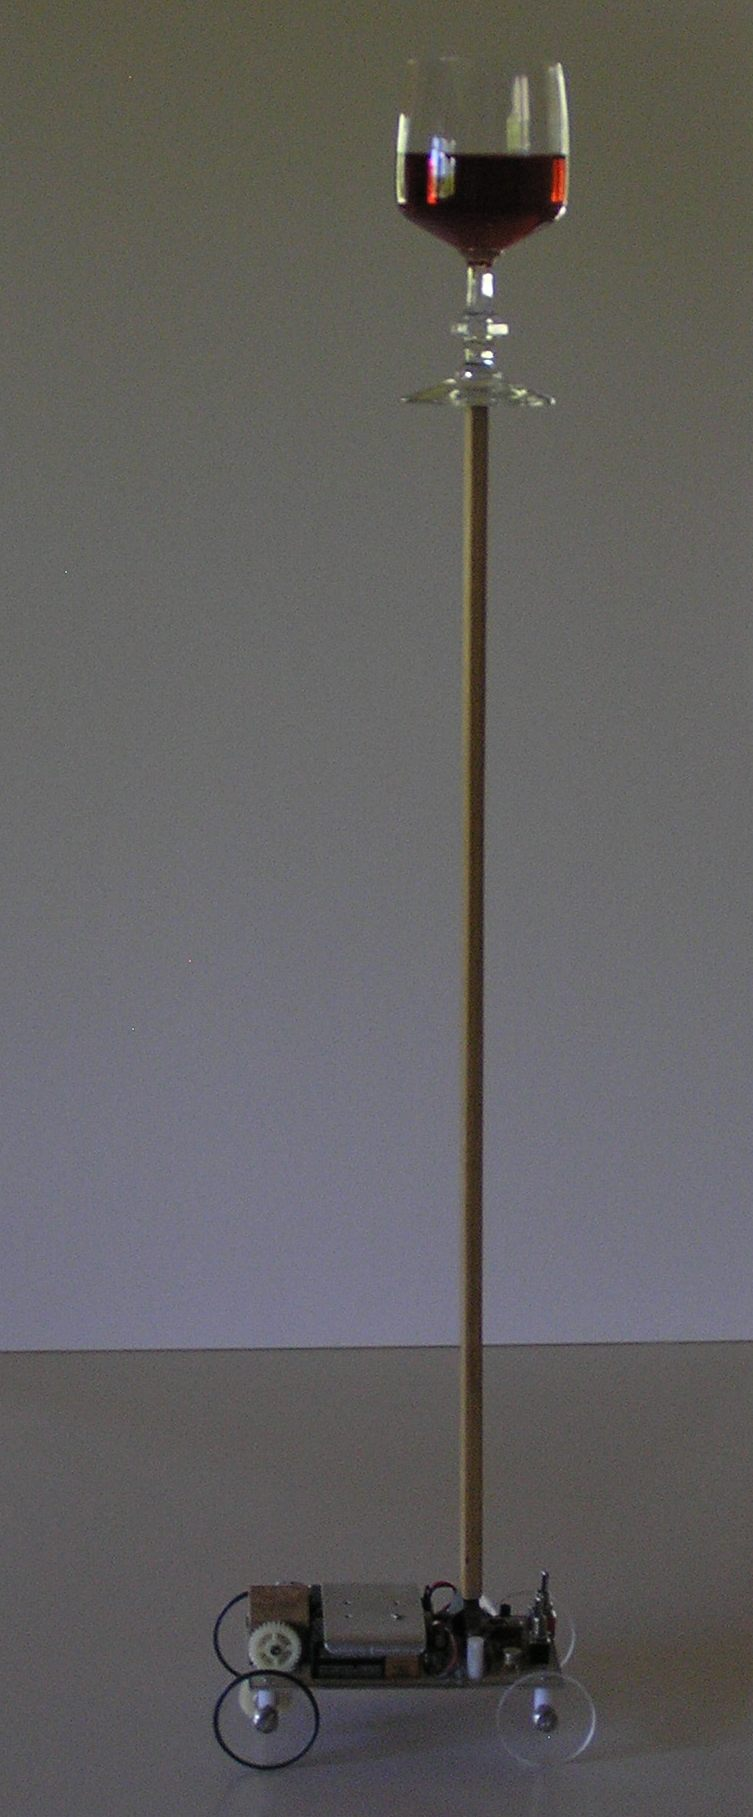
\includegraphics[scale=0.5]{images/wine.jpg} }
    \only<2> { 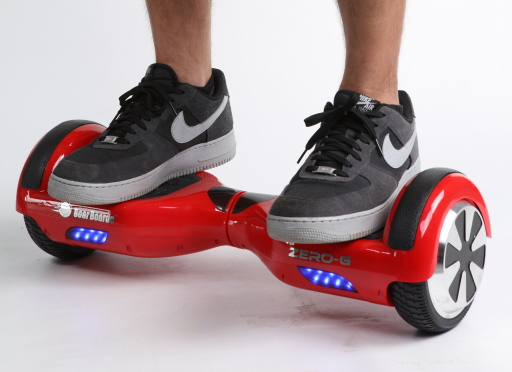
\includegraphics[scale=0.75]{images/board.png} }
    \only<3> { 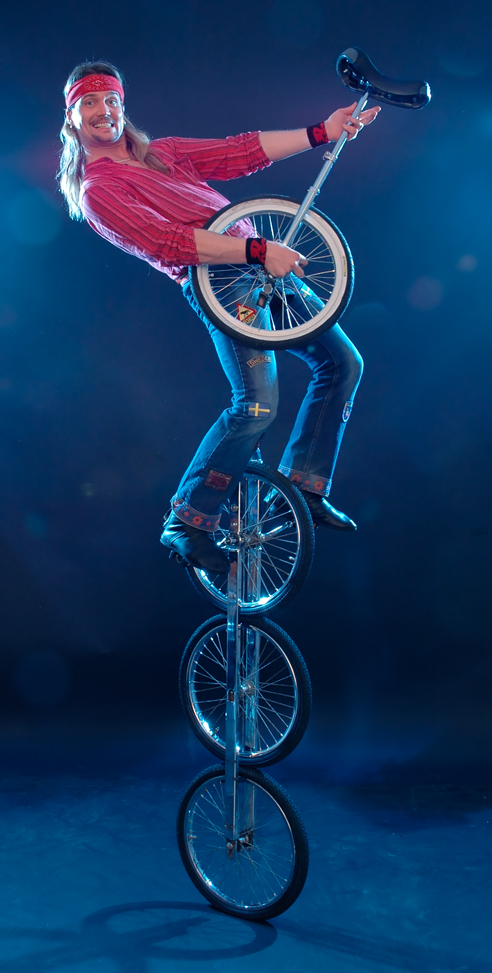
\includegraphics[scale=0.22]{images/einrad.jpg} }
    \end{center}

    \vfill

    \hrule
    {
    \tiny
    \begin{flushright}
    \only<1> { balancing cart (1976), \url{https://en.wikipedia.org/wiki/Inverted_pendulum} }
    \only<2> { hoverboard, \url{https://de.wikipedia.org/wiki/E-Board}}
    \only<3> { Einrad, \url{https://en.wikipedia.org/wiki/Unicycle} }
    \end{flushright}
    }
}

\section{Invertiertes Doppelpendel}

\frame {
    \frametitle{Doppelpendel}

    \begin{minipage}[b]{0.35\textwidth}
    \begin{center}
    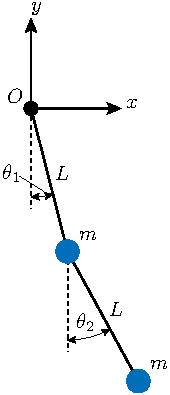
\includegraphics[scale=1.1]{images/sketch.pdf}
    \end{center}
    \end{minipage}
    \hfill
    \begin{minipage}[b]{0.6\textwidth}
	Koordinaten
    \begin{align}
    \nonumber
    x_1 &= L \sin\theta_1 \\
    \nonumber
    y_1 &= -L \cos\theta_1 \\
    \nonumber
    x_2 &= L \sin\theta_1 + L \sin\theta_2 \\
    \nonumber
    y_2 &= -L \cos\theta_1 - L \cos\theta_2
    \end{align}

    \vfill

    Lagrange-Funktion
    \begin{align}
    \nonumber
    \mathcal{L} &= T-V \\
    \nonumber
    T &= \frac{1}{2} m v^2 \\
    \nonumber
    V &= mgL \left( 3-2\cos\theta_1-\cos\theta_2\right)
    \end{align}
    \end{minipage}
}

\frame {
    \frametitle{Linearisieren um $\theta_1\approx\theta_2\approx\pi$}

    \only<1>
    {
    Kinetische Energie
    \begin{equation}
    \nonumber
    T = \frac{1}{2} m \left( \dot x_1^2 + \dot y_1^2 + \dot x_2^2 + \dot y_2^2\right)
    \approx \frac{1}{2} mL^2 \left( 2\dot\theta_1^2  + \dot\theta_2^2 + \dot\theta_1\dot\theta_2\right)
    \end{equation}

    \vfill

    Potentielle Energie ($\Delta_j \equiv \theta_j-\pi$)
    \begin{equation}
    \nonumber
    V = mgL\left(3-2\cos\theta_1-\cos\theta_2\right) = mgL\left(6-\Delta_1^2-\frac{\Delta_2^2}{2}\right)
    \end{equation}

    \vfill

    Lagrange-Funktion
    \begin{equation}
    \nonumber
    \mathcal{L} \approx \frac{1}{2} mL^2 \left( 2\dot \Delta_1^2  + \dot \Delta_2^2 + \dot \Delta_1\dot \Delta_2\right) + mgL\left( \Delta_1^2 + \frac{\Delta_2^2}{2} -6\right)
    \end{equation}
    }

    \only<2>
    {
    \vfill

    Euler-Lagrange--Gleichungen
    \begin{equation}
    \nonumber
    \frac{\mathrm{d}}{\mathrm{d}t} \frac{\partial\mathcal{L}}{\partial\dot \Delta_j} - \frac{\partial\mathcal{L}}{\partial \Delta_j} = 0
    \end{equation}

    Bewegungsgleichungen
    \begin{equation}
    \nonumber
    \frac{L}{g}
    \begin{pmatrix}
    1 & \nicefrac{1}{2} \\
    1 & 1
    \end{pmatrix}
    \begin{pmatrix}
    \ddot \Delta_1 \\ \ddot \Delta_2
    \end{pmatrix}
    =
    \begin{pmatrix}
    \Delta_1 \\ \Delta_2
    \end{pmatrix}
    \end{equation}

    \vfill

    Eigenfrequenzen
    \begin{equation}
    \nonumber
    \omega_1 = \sqrt{\frac{g}{L}} \sqrt\frac{2}{2-\sqrt{2}}, \qquad
    \omega_2 = \sqrt{\frac{g}{L}} \sqrt\frac{2}{2+\sqrt{2}}
    \end{equation}
    }
}

\frame {
    \frametitle{Normalkoordinaten}

    Kleine Abweichungen $\Delta_j\approx0$ in Normalkoordinaten
    \begin{equation}
    \nonumber
    \ddot X_j - \omega_j^2 X_j = 0, \qquad j=1,\dots,N
    \end{equation}

    \vfill

    \begin{minipage}[c]{0.5\textwidth}
    Als System 1. Ordnung
    \begin{equation}
    \nonumber
    \frac{\mathrm{d}}{\mathrm{d}t} \begin{pmatrix}
    X_j \\ Y_j
    \end{pmatrix} =
    \begin{pmatrix}
    0 & 1 \\
    \omega_j^2 & 0
    \end{pmatrix}
    \begin{pmatrix}
    X_j \\ Y_j
    \end{pmatrix}
    \end{equation}
    \vfill
    Eigenwerte
    \begin{equation}
    \nonumber
    \lambda_{1,2} = \pm\omega_j
    \end{equation}
    \end{minipage}%
    \begin{minipage}[c]{0.5\textwidth}
    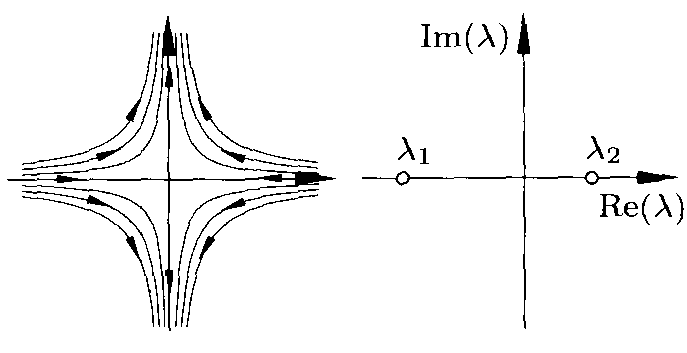
\includegraphics[scale=0.33]{images/saddle_point.png}

    \vfill

    \hrule
    \begin{flushright}
    { \tiny An Exploration of Chaos, Argyris, Faust, Haase }
    \end{flushright}
    \end{minipage}
}

\frame {
    \frametitle{Stabilisieren}

    Aufhängung $O$ oszilliere nun mit Frequenz $\omega_0$ und Amplitude $\epsilon$ nach oben und unten
    \begin{equation}
    \nonumber
    \ddot X_j - \omega_j^2 \left( 1+\frac{\epsilon \omega_0^2}{g}\cos{(\omega_0 t)} \right)X_j = 0, \qquad j=1,\dots,N
    \end{equation}

    \vfill

    Reskalieren mit $\tau = \omega_0 t$
    \begin{equation}
    \nonumber
    \frac{\mathrm{d}^2 X_j}{\mathrm{d}\tau^2} + \left( \alpha_j+\beta_j\cos\tau \right) X_j = 0, \qquad j=1,\dots,N
    \end{equation}
    \begin{equation}
    \nonumber
    \text{mit} \qquad \alpha_j = - \omega_j^2/\omega_0^2, \quad \beta_j = -\omega_j^2\epsilon/g
    \end{equation}

    \only<2>
    {
    \vfill
    \begin{center}
    \color{purple}
    \Large
    $\Rightarrow$ $N$ ungekoppelte Mathieu-Gleichungen
    \end{center}
    }
}

\section{Mathieu-Gleichung}

\frame {
    \frametitle{Mathieu-Gleichung}

    Mathieu-Gleichung
    \begin{equation}
    \nonumber
    \ddot y(t) + \left(\alpha+\beta\cos t\right) y(t) = 0
    \end{equation}

    \vfill

    Eigenschaften
    \begin{itemize}
    \item linear
    \item homogen
    \item $2\pi$-periodisch
    \end{itemize}
}

\frame {
    \frametitle{Floquet-Theorem}

    {\color{purple}Theorem: }Jede Fundamentalmatrix $\Phi$ von
    $$\dot y(t) = \mathcal{L}(t) y(t)$$
    mit stetiger $\omega$-periodischer Koeffizientenmatrix $\mathcal{L}$ lässt sich als
    $$\Phi(t) = \mathcal{P}(t) \exp(\mathcal{R}t)$$
    schreiben, wobei $\mathcal{P}$ $\omega$-periodisch und $\mathcal{R}$ konstant.

    \vfill

    {\color{purple}Definition:} Es gilt $\Phi(t+T) = \Phi(t)\mathcal{B}$ und die Eigenwerte $\lambda_j$ von $\mathcal{B}$ heißen charakteristische Multiplikatoren.
}

\frame {
    \frametitle{Floquet-Theorem (2)}

    {\color{purple}Lemma:} Sei $\lambda_j$ ein charakteristischer Multiplikator, dann existiert eine Lösung
    $$y(t+T)=\lambda_j y(t)\,.$$

    \vfill

    {\color{purple}Stabilität:} Falls $|\lambda_j|>1$, dann divergiert $y(t)$ für $t\to\infty$.

    \vfill

    Numerisch:
    \begin{enumerate}
    \item Berechne Propagator $U(t+T,t)$
    \item Berechne Eigenwerte $\lambda_j$ von $U(t+T,t)$
    \item Falls alle Eigenwerte $|\lambda_j| \le 1$ $\rightarrow$ stabil
    \end{enumerate}
}

\frame {
    \frametitle{Stabilität Mathieu-Gleichung}

    \begin{center}
    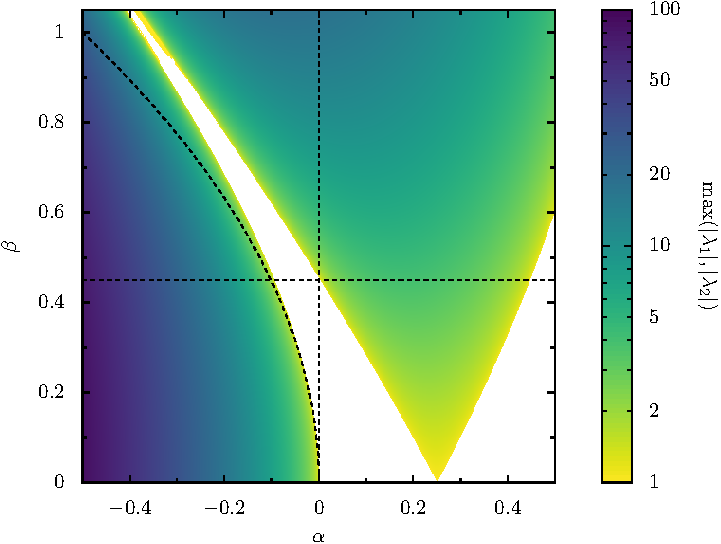
\includegraphics[scale=0.9]{plots/mathieu.pdf}
    \end{center}
}

\frame {
    \frametitle{Stabilität invertiertes $N$-Pendel}

    \begin{minipage}{0.6\textwidth}
    {\color{purple}Idee:} Wähle $\epsilon$, $\omega_0$ so, dass alle Punkte
    $$(\alpha,\beta) = (-\omega_j^2/\omega_0^2, \omega_j^2\epsilon/g)$$
    im stabilen Bereich liegen.
    \end{minipage}
    \begin{minipage}{0.34\textwidth}
    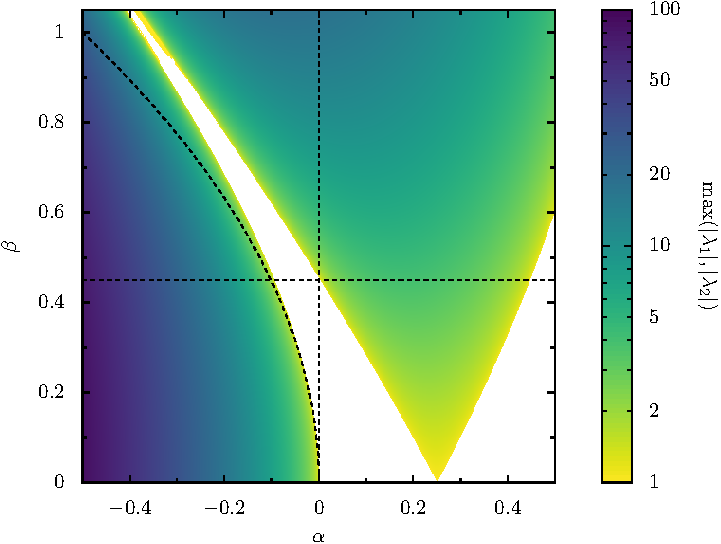
\includegraphics[scale=0.4]{plots/mathieu.pdf}
    \end{minipage}


    \vfill

    \textcolor{purple}{Hochfrequenz-Limes:} $\omega_0^2 \gg \omega_\mathrm{max}^2$
    \begin{align}
    \nonumber
    \alpha = -\frac{\omega_j^2}{\omega_0^2} > -\frac{\beta^2}{2} = -\frac{\omega_j^4\epsilon^2}{2g^2} \quad &\Rightarrow \quad \frac{\sqrt{2} g}{\omega_0 \omega_j} < \epsilon \\
    \nonumber
    \beta = \frac{\omega_j^2\epsilon}{g} < \epsilon \quad &\Rightarrow \quad \epsilon < 0.45 \frac{g}{\omega_j^2}
    \end{align}

    {
        \Large
        \color{purple}
    $$\Rightarrow \frac{\sqrt{2} g}{\omega_0 \, \omega_\mathrm{min}} < \epsilon < 0.45 \frac{g}{\omega_\mathrm{max}^2}$$
    }
}

\section{Beispiele}

\frame {
    \frametitle{invertiertes Doppelpendel}

    Stabilitätsbedingung

    \begin{itemize}
    \item für $m_1=m_2=m$:
    $$\sqrt{\frac{g}{L}} \frac{\sqrt{2+\sqrt{2}}}{\omega_0} < \frac{\epsilon}{L} < 0.45 \frac{2-\sqrt{2}}{2}$$

    \item für beliebige Massenverhältnisse ($m_1$ mit $O$ verbunden):
    $$\sqrt{\frac{g}{L}} \frac{\sqrt{2+2\sqrt{\mu}}}{\omega_0} < \frac{\epsilon}{L} < 0.45 (1-\sqrt{\mu})$$
    mit $$\mu=\frac{m_2}{m_1+m_2}$$
    \end{itemize}
}

\frame {
    \frametitle{invertiertes $N$-Pendel}

    \begin{center}
    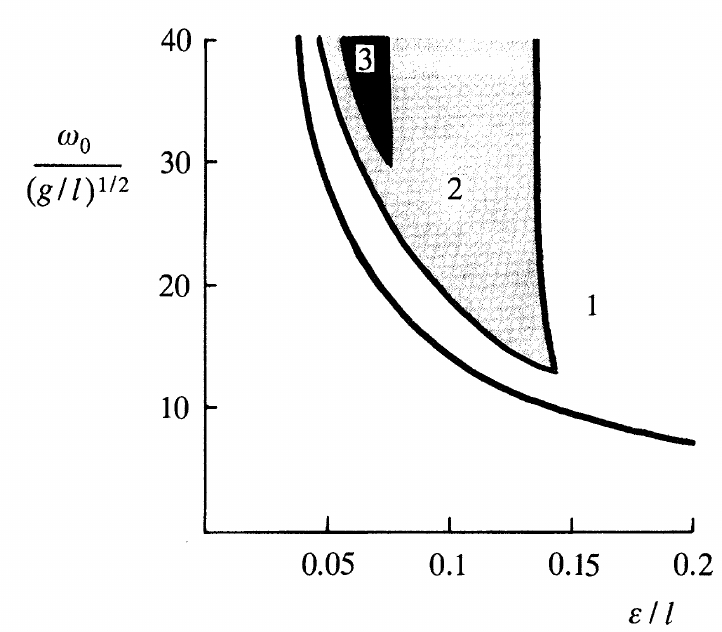
\includegraphics[scale=0.45]{images/npendula.png}
    \end{center}

    \hrule
    {
    \tiny
    \begin{flushright}
    D. J. Acheson, \textbf{A pendulum theorem}, The Royal Society (1993)
    \end{flushright}
    }
}

\frame {
    \frametitle{Indischer Seiltrick}

    \begin{center}
    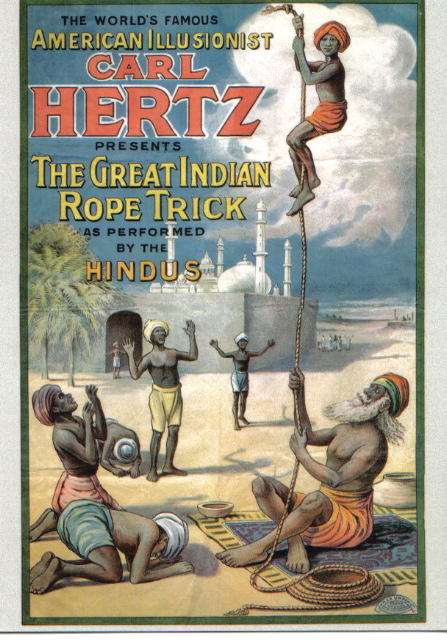
\includegraphics[height=0.83\textheight]{images/Indian-Rope-Trick.jpg} \quad
    \includegraphics[height=0.83\textheight]{images/Indian-Rope-Trick_2.jpg}
    \end{center}

    \vfill

    \hrule
    {
    \tiny
    \begin{flushright}
    Quelle: \url{https://en.wikipedia.org/wiki/Indian_rope_trick}
    \end{flushright}
    }
}

\frame {
    \frametitle{Indischer Seiltrick}

    \only<1>
    {
    Eigenfrequenzen eines $N$-Pendels
    $$\omega_j = \sqrt{\xi_j \, \frac{g}{L}}, \qquad j=1,\dots,N$$

    \vfill

    Asymptotische Entwicklung von $\xi_j$ für $N\gg 1$
    $$\xi_j \simeq \nicefrac{\chi_j^2}{4N}, \qquad \chi_j \simeq \left(N-\nicefrac{1}{4}\right)\pi$$

    \vfill
    }

    Größte/kleinste Eigenfrequenz
    $$\omega_\mathrm{min} \approx 1.2\sqrt{\frac{g}{N L}}, \qquad \omega_\mathrm{max} \approx \frac{\pi}{2} \left(N-\nicefrac{1}{4}\right) \sqrt{\frac{g}{N L}}$$

    \only<2,3>
    {
    \vfill

    Stabilitätsbedingung
    $$\frac{1.18}{\omega_0} \sqrt{\frac{g}{N L}} < \frac{\epsilon}{N L} < \frac{0.182}{\left(N-\nicefrac{1}{4}\right)^2}$$
    }

    \only<3>
    {
    \vfill
    \begin{center}
    \color{purple}
    \Large
    $\Rightarrow$ für $N\gg1$ immer schwieriger zu erfüllen
    \end{center}
    }
}

\frame[c] {
    \frametitle{Vielen Dank für die Aufmerksamkeit}
    \begin{center}
    {
        
\includegraphics[height=0.4\textheight]{images/pink.png}
    }
    \end{center}

    \vfill
    \vfill
    \vfill
    \vfill
    \vfill

    Bibliographie
    \begin{itemize}
    \item \hyperlink{http://dx.doi.org/10.1098/rspa.1993.0142}{D. J. Acheson, \textbf{A pendulum theorem}, The Royal Society (1993)}
    \end{itemize}
}

\end{document}
